\documentclass[10pt,a4paper]{article}
\usepackage[utf8]{inputenc}
\usepackage[margin=0.65in]{geometry}
\usepackage{tikz}
\usepackage{float}
\usepackage{adjustbox}
\usetikzlibrary{shapes.geometric, arrows.meta, positioning, calc, fit, backgrounds}

% Styles shared with the playbook figure
\tikzstyle{startstop} = [rectangle, rounded corners, minimum height=0.75cm, text centered,
  draw=black, fill=black!5, text=black, text width=4.2cm, font=\scriptsize\bfseries]
\tikzstyle{process} = [rectangle, minimum height=0.7cm, text centered, text width=3.2cm,
  draw=black, fill=white, text=black, font=\scriptsize]
\tikzstyle{review} = [process, line width=1.1pt, fill=black!8]
\tikzstyle{explore} = [process, dashed]
\tikzstyle{note} = [process, draw=black!50, text=black!80, font=\tiny, text width=2.6cm]
\tikzstyle{group} = [draw=black!60, dashed, rounded corners, inner sep=0.22cm]
\tikzstyle{grouplabel} = [font=\tiny, anchor=north west, inner sep=2pt]
\tikzstyle{arrow} = [thick, ->, >=stealth]
\tikzstyle{thinarrow} = [->, >=stealth, draw=black!55]

\begin{document}

\begin{figure}[H]
\centering
\begin{adjustbox}{max width=\textwidth}
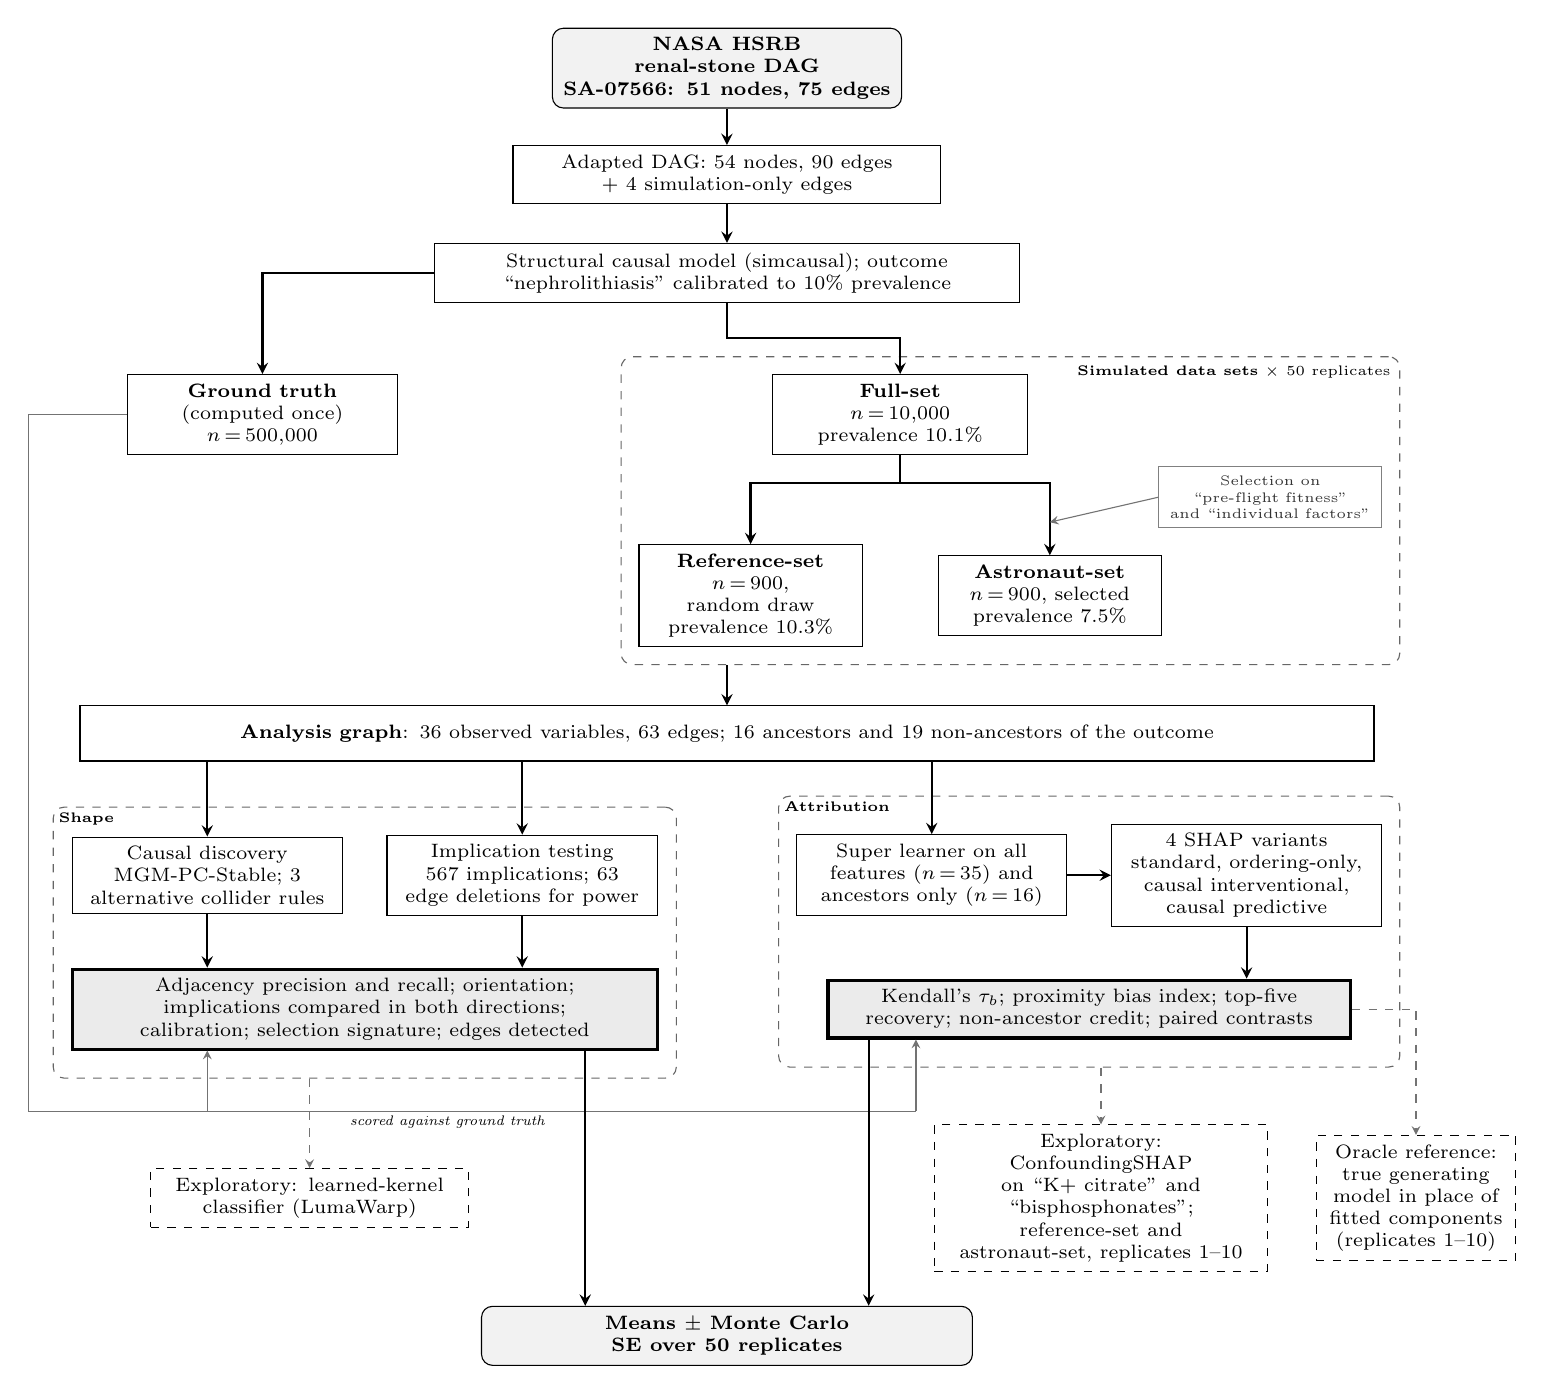
\begin{tikzpicture}[every node/.append style={execute at begin node={\hyphenpenalty=10000\exhyphenpenalty=10000\relax}}]

  % --- Source and simulation ---
  \node (src) [startstop] at (0,0) {NASA HSRB renal-stone DAG\\SA-07566: 51 nodes, 75 edges};
  \node (adapt) [process, text width=5.2cm] at (0,-1.35) {Adapted DAG: 54 nodes, 90 edges\\+ 4 simulation-only edges};
  \node (sim) [process, text width=7.2cm] at (0,-2.6)
    {Structural causal model (simcausal); outcome ``nephrolithiasis'' calibrated to 10\% prevalence};
  \draw [arrow] (src) -- (adapt);
  \draw [arrow] (adapt) -- (sim);

  % --- Ground truth ---
  \node (truth) [process, text width=3.2cm] at (-5.9,-4.4) {\textbf{Ground truth}\\(computed once)\\$n\,{=}\,500{,}000$};
  \draw [arrow] (sim.west) -| (truth.north);

  % --- Simulated data sets (attrition style) ---
  \node (full) [process, text width=3.0cm] at (2.2,-4.4) {\textbf{Full-set}\\$n\,{=}\,10{,}000$\\prevalence 10.1\%};
  \node (sel) [note] at (6.9,-5.45) {Selection on ``pre-flight fitness'' and ``individual factors''};
  \node (ref) [process, text width=2.6cm] at (0.3,-6.7) {\textbf{Reference-set}\\$n\,{=}\,900$, random draw\\prevalence 10.3\%};
  \node (astro) [process, text width=2.6cm] at (4.1,-6.7) {\textbf{Astronaut-set}\\$n\,{=}\,900$, selected\\prevalence 7.5\%};
  \draw [arrow] (full.south) -- ++(0,-0.35) -| (ref.north);
  \draw [arrow] (full.south) -- ++(0,-0.35) -| (astro.north);
  \draw [thinarrow] (sel.west) -- ($(astro.north)+(0,0.42)$);
  \begin{scope}[on background layer]
    \node (reps) [group, fit=(full) (ref) (astro) (sel)] {};
  \end{scope}
  \node [font=\tiny, anchor=north east] at (reps.north east) {\textbf{Simulated data sets} $\times$ 50 replicates};
  \draw [arrow] (sim.south) -- ++(0,-0.45) -| (full.north);

  % --- Analysis graph ---
  \node (ag) [process, text width=16.2cm] at (0,-8.45)
    {\textbf{Analysis graph}: 36 observed variables, 63 edges; 16 ancestors and 19 non-ancestors of the outcome};
  \draw [arrow] (reps.south -| ag.north) -- (ag.north);

  % --- Shape arm ---
  \node (disc) [process] at (-6.6,-10.25) {Causal discovery\\MGM-PC-Stable; 3 alternative collider rules};
  \node (impl) [process] at (-2.6,-10.25) {Implication testing\\567 implications; 63 edge deletions for power};
  \node (shapescore) [review, text width=7.2cm] at (-4.6,-11.95)
    {Adjacency precision and recall; orientation; implications compared in both directions; calibration; selection signature; edges detected};
  \draw [arrow] (ag.south -| disc.north) -- (disc.north);
  \draw [arrow] (ag.south -| impl.north) -- (impl.north);
  \draw [arrow] (disc.south) -- (disc.south |- shapescore.north);
  \draw [arrow] (impl.south) -- (impl.south |- shapescore.north);
  \begin{scope}[on background layer]
    \node (shapebox) [group, fit=(disc) (impl) (shapescore), inner ysep=0.35cm] {};
  \end{scope}
  \node [grouplabel] at (shapebox.north west) {\textbf{Shape}};

  % --- Attribution arm ---
  \node (sl) [process] at (2.6,-10.25) {Super learner on all features ($n\,{=}\,35$) and ancestors only ($n\,{=}\,16$)};
  \node (shap) [process] at (6.6,-10.25) {4 SHAP variants\\standard, ordering-only, causal interventional, causal predictive};
  \node (attrscore) [review, text width=6.4cm] at (4.6,-11.95)
    {Kendall's $\tau_b$; proximity bias index; top-five recovery; non-ancestor credit; paired contrasts};
  \draw [arrow] (ag.south -| sl.north) -- (sl.north);
  \draw [arrow] (sl) -- (shap);
  \draw [arrow] (shap.south) -- (shap.south |- attrscore.north);
  \begin{scope}[on background layer]
    \node (attrbox) [group, fit=(sl) (shap) (attrscore), inner ysep=0.35cm] {};
  \end{scope}
  \node [grouplabel] at (attrbox.north west) {\textbf{Attribution}};

  % --- Ground truth feeds both scored boxes ---
  \coordinate (bus) at (0,-13.25);
  \draw [draw=black!55] (truth.west) -- ++(-1.25,0) |- (2.4,0 |- bus);
  \draw [thinarrow] (-6.6,0 |- bus) -- (-6.6,0 |- shapescore.south);
  \draw [thinarrow] (2.4,0 |- bus) -- (2.4,0 |- attrscore.south);
  \node [font=\tiny\itshape, anchor=north, inner sep=1.5pt] at (-3.55,0 |- bus) {scored against ground truth};

  % --- Exploratory and diagnostic analyses ---
  \node (luma) [explore, text width=3.8cm] at (-5.3,-14.35) {Exploratory: learned-kernel classifier (LumaWarp)};
  \node (cshap) [explore, text width=4.0cm] at (4.75,-14.35)
    {Exploratory: ConfoundingSHAP on ``K+~citrate'' and ``bisphosphonates''; reference-set and astronaut-set, replicates 1--10};
  \draw [thinarrow, dashed] (shapebox.south -| luma.north) -- (luma.north);
  \draw [thinarrow, dashed] (attrbox.south -| cshap.north) -- (cshap.north);
  % OPTIONAL: oracle reference (delete this node and its arrow to drop it)
  \node (oracle) [explore, text width=2.3cm] at (8.75,-14.35) {Oracle reference: true generating model in place of fitted components (replicates 1--10)};
  \draw [thinarrow, dashed] (attrscore.east) -| (oracle.north);

  % --- Output ---
  \node (out) [startstop, text width=6.0cm] at (0,-16.1) {Means $\pm$ Monte Carlo SE over 50 replicates};
  \draw [arrow] (-1.8,0 |- shapescore.south) -- (-1.8,0 |- out.north);
  \draw [arrow] (1.8,0 |- attrscore.south) -- (1.8,0 |- out.north);

\end{tikzpicture}
\end{adjustbox}

\vspace{0.1cm}
{\raggedright\scriptsize \hyphenpenalty=10000\exhyphenpenalty=10000 Counts are per replicate unless stated.\par}
\end{figure}

\end{document}
